\section{Technical Stack}
\subsection{Technologies Used}
For the platform to distribute our solution on, it was felt that a mobile solution was the most applicable. Ideally apps exist on both the Google Play Store as well as the Apple Apple Store, however due to time constraints, we chose to stick to one platform, that being iOS. A large part of that decision was doing to members of the group having experience with developing iOS applications and thus this would ultimately speed up development. Objective-C was chosen for development due to this past experience, however for future maintainers may decide to switch over to Swift, there are certainly benefits this language, but it did not make sense at the time.
\subsection{Implementation}
\subsubsection{User Interface Design Process}
The first step after identifying iOS as the most suitable platform, was to convert the product requirements to user experience flows. From there the design process begins with various steps:
\begin{enumerate}
    \item Ideation
    \item Sketches
    \item Lo-fi mockups
    \item Design Reviews
\end{enumerate}
One aspect of design that was important to keep up with was the Apple Human Interface Guidelines\footnote{\url{https://developer.apple.com/design/human-interface-guidelines/}}. Apple is quite strict on ensuring that apps on their plateform follow this guidelines. There are six main design principles that need to be followed: Aesthetic Integrity, Consistency, Direct Manipulation, Feedback, Metaphors and User Control.
\newline \newline
For building our these user experiences it was chosen to use a combination of Xcode Storyboards and as well as programming flows in code. In the future moving to SwiftUI\footnote{\url{https://developer.apple.com/xcode/swiftui/}} would be a good decision.
\begin{figure}[h]
\centering
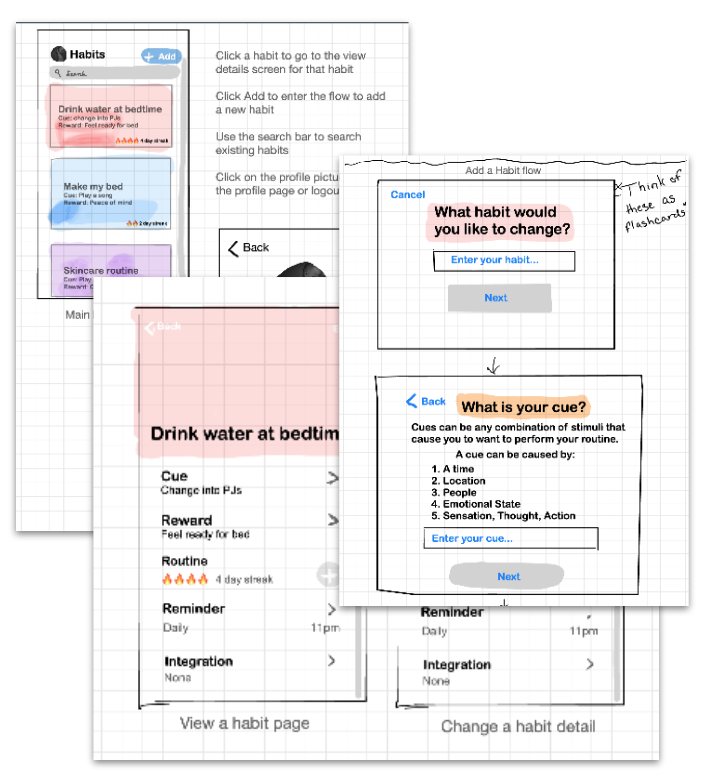
\includegraphics[width=0.7\textwidth]{images/mockups.png}
\caption{Early lo-fi mockups}
\end{figure}
\subsubsection{Backend and Database Services}
The current version of the iOS app utilizes Apple's CoreData and CloudKit services opposed to a tradition backend. CoreData is a local store that is effectively wrapper around SQLite. It is fairly light-weight and has great development tools in Xcode for building database schemas and having the ORM models in your codebase be generated automatically. CoreData stores all user infomration on the local storage of their iOS device, which is great from a security standpoint. CloudKit on the other hand, is used to sync data between all of the devices associated with a user's iCloud account. By using CloudKit habits added on someones iPhone, get pushed to their iPad, or even macOS devices (if there was a macOS app). Using both of these technologies was great, they were fairly easy to implement and get working consistently. The only downside is you are heavily locking your code into the Apple ecosystem. For a future iteration of this project, it may be worth while moving other to a dedicated backend solution, especially if there exists desire to create an Android version alongside the iOS.
\begin{figure}[h]
\centering
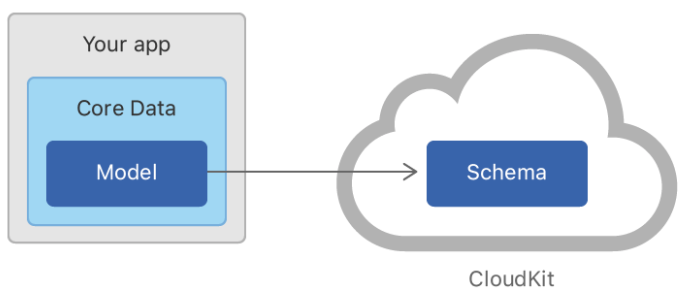
\includegraphics[width=0.55\textwidth]{images/cloudkit.png}
\caption{Basic CloudKit layout}
\end{figure}
\subsubsection{Security and Privacy}
\begin{itemize}
    \item \textbf{Sign in with Apple:} This feature allows users to have peace of mind about their privacy. "Data collection is limited to the user’s name and email address, and Apple’s private email relay lets users receive email even if they prefer to keep their address private. Apple will not track users as they interact with your app."\footnote{\url{https://developer.apple.com/sign-in-with-apple/}}. A benefit to using this feature, is that it moves the concern of data privacy from the application to Apple. Apple takes privacy very seriously so to have user data protected by their systems versus the applications is a great way to decrease the liability exposure of the application.
    \item \textbf{Habit Data:} As mentioned in section 4.2.2 the application utilizes Apple CoreData and CloudKit for handling user data. While CoreData stores data locally on a user's device, CloudKit uses iCloud syncing to transmit information, thus the potential for a users habit data to get compromised. One easy solution is to allow users to toggle on/off CloudKit in settings. Regardless of whether multi-device sync is enabled or not, the application backend is never able to see a users habit information that they enter, thereby removing another potential liability for the application.
\end{itemize}

\subsection{Potential Expansions}
If implementing these in a future expansion, ensure that there is sufficient justification to do so. Adding features for "the sake of adding features" or "because we need more technical complexity" is not valid justification. Excess bloat was one of the things that was found to be detrimental to many of the habit tracking apps on App Store's today. The following are some ideas that were brought up during the development process but were never implemented.
\subsubsection{Health Data}
A lot of people try to make health related habit improvement. Drink more water, exercise more and eating less processed foods are some good examples. Thus the can take advantage of health data that may be stored on a users phone. Data from places such as the built in pedometer, water tracking and even 3rd party apps like MyFitnessPal, could be used. This could be extended to an Apple Watch companion app as well, which would make this integration more accurate and more powerful. For example the heart rate sensor in the watch can auto detect periods of exercise, so if one users habits involved "go for a run during lunch break", the watch could auto detect and inform the app that the user has done their new routine.
\subsubsection{Financial Data}
Services like Plaid\footnote{\url{https://plaid.com/what-is-plaid/}} are easy for developers to use and can allow users to integrate with over 11,000 different financial institutions. This could be used to help people who want to create financially oriented habits like save and invest money. On top of Plaid, another app that was discovered, Alpaca \footnote{\url{https://alpaca.markets/}} is an online broker that has no market interface or GUI of any kind. You have to provide the full interface in Python yourself. It could be utilized to have users do automatic investing that apps like Acorns\footnote{\url{https://www.acorns.com/}} have been doing for years.
\subsubsection{Location Data}
Location data could be utilized by the app to assist in managing habits that involve a specific location as part of their cue. For instance the app could send a push notification when a user gets to a certain point in their commute to tell them to listen to an educational e-book or when they go to the grocery store, make sure that they buy healthy foods.
\subsubsection{Spotify API}
Spotify\footnote{\url{https://developer.spotify.com/documentation/web-api/}} has an API that can be used to play music clips within an application, as well as a variety of other features. This would not investigated into much detail, but there was motive that it may be useful for people that who have a music based queue. Ultimately the idea was dropped as it felt too niche if a cue to focus on for an early rendition of the app.
\subsubsection{IFTTT}
"IF This Then That"\footnote{\url{https://ifttt.com/}} is a service that can be used to register webhooks with actions in a wide variety of application. It was not investigated in very much detail, but it could potentially be of use. 